\section{Simulation Studies : Performance and Efficiency of KAC}
\label{sec:results}
% 
% In this section we present experimental results from our implementations of the extended generalized scheme using Tate pairings on BN-curves using $256$ bit primes \cite{ghosh2013secure}. All our experiments have been carried out on an AMD Opteron (TM) Processor $6272\times16$ with a clock frequency $1.4$ GHz.
% 
% \subsection{Space and Time Complexities}
% 
% \begin{table}[!t]
% \centering
% \captionsetup{font=scriptsize}
% \caption{Space Complexities}
% \label{tab:space}
% \scalebox{0.6}{
% \begin{tabular}{|c|c|c|c|c|c|c|c|}
%   \hline 
%   $n_1$ & $n_2$ & $param$ & $PK$ & $msk$ & $K_{\mathcal{S}}$ & $U$ & Total\\
%   & & (in bytes) & (in bytes) & (in bytes) & (in bytes) & (in bytes) & (in KB)\\\hline\hline
%   1 & 100 & 16112 & 144 & 40 & 72 & 64 & 16.046875\\\hline
%   2 & 50 & 8112 & 240 & 56 & 120 & 64 & 8.390625\\\hline
%   4 & 25 & 4112 & 432 & 88 & 216 & 64 & 4.796875\\\hline
%   5 & 20 & 3312 & 528 & 104 & 264 & 64 & 4.171875\\\hline
%   \textbf{10} & \textbf{10} & \textbf{1712} & \textbf{1008} & \textbf{184} & \textbf{504} & \textbf{64} & \textbf{3.390625}\\\hline
%   20 & 5 & 912 & 1968 & 344 & 984 & 64 & 4.171875\\\hline
%   25 & 4 & 752 & 2448 & 424 & 1224 & 64 & 4.796875\\\hline
%   50 & 2 & 432 & 4848 & 824 & 2424 & 64 & 8.390625\\\hline
%   100 & 1 & 272 & 9648 & 1624 & 4824 & 64 & 16.046875\\\hline
%   \hline
% \end{tabular}}
% \end{table}
% 
% \begin{table}[!t]
% \centering
% \captionsetup{font=scriptsize}
% \caption{Time Complexities}
% \label{tab:time}
% \scalebox{0.6}{
% % \begin{tabular}{|c|c|c|c|c|c|}
% \begin{tabular}{|c|c|c|c|c|c|c|c|}
%   \hline 
%   $n_1$ & $n_2$ & $SetUp$ & $KeyGen$ & $Encrypt$ & $Extract$ & $Decrypt$ & Total\\
%   & & (in clock cycles) & (in clock cycles) & (in clock cycles) & (in clock cycles) & (in clock cycles) & (in clock cycles)\\\hline\hline
%   1 & 100 & 2920000 & 10000 & 7932000 & 47000 & 16095000 & 27004100\\\hline 
%   2 & 50 & 1410000 & 30000 & 8065000 & 53000 & 16110000 & 25668000\\\hline
%   4 & 25 & 690000 & 60000 & 8130000 & 81000 & 16284000 & 25245000\\\hline
%   5 & 20 & 590000 & 70000 & 8091000 & 96000 & 16379000 & 25226000\\\hline
%   \textbf{10} & \textbf{10} & \textbf{280000} & \textbf{140000} & \textbf{7957000} & \textbf{170000} & \textbf{16049000} & \textbf{25136000}\\\hline
%   20 & 	5 & 130000 & 270000 & 8070000 & 320000 & 16361000 & 25151000\\\hline
%   25 & 4 & 120000 & 350000 & 8256000 & 370000 & 16239000 & 25836000\\\hline
%   50 & 2 & 50000 & 680000 & 8265000 & 712000 & 16398000 & 26105000\\\hline
%   100 & 1 & 30000 & 1360000 & 8201000 & 1315000 & 16142000 & 27048000\\\hline
% 
%   \hline
% \end{tabular}}
% \end{table}
% % \vspace{-2mm}
% 
% Table \ref{tab:space} summarizes the space requirements for various parameters of the scheme for different values of $(n_1,n_2)$. The results have been averaged over $100$ randomly chosen subsets of the $n=100$ ciphertext classes. Table \ref{tab:time} summarizes the time complexity for various operations of the scheme for different values of $(n_1,n_2)$. The results have been averaged over $100$ randomly chosen subsets of the $n=100$ ciphertext classes. The encryption and decryption operation complexities are further averaged over $10$ message transmissions corresponding to each subset. We point out that both the overall space and time requirements are minimum for $n_1=n_2=10=\surd n$, which proves the usefulnesss of the generaalization.
% 
% \subsection{Comparison with Hierarchy Based Schemes}
% % \vspace{-2mm}
% \begin{figure*}[!t]
% \captionsetup{font=scriptsize}
% \centering
% % \caption{Simulation results}
% 
% % n_1:n_2	0.1	0.2	0.3	0.4	0.5	0.6	0.7	0.8	0.9
% % 1:100	0.1	0.05	0.0333333	0.025	0.02	0.0166667	0.0142857	0.0125	0.0111111
% % 2:50	0.2	0.1	0.0666667	0.05	0.04	0.0333333	0.0285714	0.025	0.0222222
% % 4:25	0.37	0.2	0.133333	0.1	0.08	0.0666667	0.0571429	0.05	0.0497512
% % 5:20	0.46	0.245	0.166667	0.125	0.1	0.0833333	0.0714286	0.0640205	0.0685871
% % 10:10	0.69	0.465	0.323333	0.245	0.2	0.166667	0.150602	0.135685	0.179211
% % 20:5	0.82	0.66	0.57	0.467172	0.419565	0.367647	0.34965	0.340136	0.454545
% % 25:4	0.9	0.715736	0.656566	0.578534	0.5141	0.481928	0.476654	0.497018	0.617284
% % 50:2	1	1	1	1	1	1	1	1	1
% % 100:1	1	1	1	1	1	1	1	1	1
% 
% \begin{subfigure}{0.5\textwidth}
% \captionsetup{font=scriptsize}
% \centering
% % \hspace*{-2.13 cm}
% \begin{tikzpicture}[scale = 0.65]
% 	 \begin{axis}[
% 	 		xlabel=Subset Size (as a fraction of total classes),
% 	 		ylabel=Ratio of Key Size (Aggregate/Hierarchical),
% % 	 		nolegend
% 	 		legend pos={north west}
% 	 		]
% 	 \addplot plot coordinates{
% 	 	(0.1,0.1)
% 		(0.2,0.05)
% 		(0.3,0.0333)
% 		(0.4,0.025)
% 		(0.5,0.02)
% 		(0.6,0.0167)
% 		(0.7,0.0143)
% 		(0.8,0.0125)
% 		(0.9,0.111)
% 	 };
% 	 %\addlegendentry{$n_1=1$, $n_2=100$}
% 	 \addplot plot coordinates{
% 	 	(0.1,0.2)
% 		(0.2,0.1)
% 		(0.3,0.067)
% 		(0.4,0.05)
% 		(0.5,0.04)
% 		(0.6,0.033)
% 		(0.7,0.0287)
% 		(0.8,0.025)
% 		(0.9,0.22)
% 	 };
% 	 %\addlegendentry{$n_1=2$, $n_2=50$}
% 	 \addplot plot coordinates{
% % 	 0.37	0.2	0.133333	0.1	0.08	0.0666667	0.0571429	0.05	0.0497512
% 	 	(0.1,0.37)
% 		(0.2,0.2)
% 		(0.3,0.1333)
% 		(0.4,0.1)
% 		(0.5,0.08)
% 		(0.6,0.067)
% 		(0.7,0.057)
% 		(0.8,0.05)
% 		(0.9,0.049)
% 	 };
% 	 %\addlegendentry{$n_1=4$, $n_2=25$}
% 	 \addplot plot coordinates{
% % 	 0.46	0.245	0.166667	0.125	0.1	0.0833333	0.0714286	0.0640205	0.0685871
% 	 	(0.1,0.46)
% 		(0.2,0.245)
% 		(0.3,0.1667)
% 		(0.4,0.125)
% 		(0.5,0.1)
% 		(0.6,0.083)
% 		(0.7,0.0714)
% 		(0.8,0.064)
% 		(0.9,0.069)
% % 		(0.9,0111)
% 	 };
% 	 %\addlegendentry{$n_1=5$, $n_2=20$}
% 	 \addplot plot coordinates{
% % 	 0.69	0.465	0.323333	0.245	0.2	0.166667	0.150602	0.135685	0.179211
% 	 	(0.1,0.69)
% 		(0.2,0.465)
% 		(0.3,0.323)
% 		(0.4,0.245)
% 		(0.5,0.2)
% 		(0.6,0.167)
% 		(0.7,0.150)
% 		(0.8,0.136)
% 		(0.9,0.179)
% 	 };
% 	 %\addlegendentry{$n_1=10$, $n_2=10$}
% % 	 0.82	0.66	0.57	0.467172	0.419565	0.367647	0.34965	0.340136	0.454545
% 	 \addplot plot coordinates{
% 	 	(0.1,0.82)
% 		(0.2,0.66)
% 		(0.3,0.57)
% 		(0.4,0.47)
% 		(0.5,0.42)
% 		(0.6,0.37)
% 		(0.7,0.35)
% 		(0.8,0.34)
% 		(0.9,0.45)
% 	 };
% 	 %\addlegendentry{$n_1=20$, $n_2=5$}
% 	 \addplot plot coordinates{
% % 	 0.9	0.715736	0.656566	0.578534	0.5141	0.481928	0.476654	0.497018	0.617284
% 	 	(0.1,0.9)
% 		(0.2,0.72)
% 		(0.3,0.66)
% 		(0.4,0.58)
% 		(0.5,0.51)
% 		(0.6,0.48)
% 		(0.7,0.47)
% 		(0.8,0.49)
% 		(0.9,0.61)
% 	 };
% 	 %\addlegendentry{$n_1=25$, $n_2=4$}
% 	 \addplot plot coordinates{
% 	 	(0.1,1)
% 		(0.2,1)
% 		(0.3,1)
% 		(0.4,1)
% 		(0.5,1)
% 		(0.6,1)
% 		(0.7,1)
% 		(0.8,1)
% 		(0.9,1)
% 	 };
% 	 %\addlegendentry{$(n_1=50$, $n_2=2)$ $\&$ $(n_1=100, n_2=1)$}
% 	 
% 	 
% \end{axis}
% \end{tikzpicture}
% \end{subfigure}%
% \begin{subfigure}{0.5\textwidth}
% \captionsetup{font=scriptsize}
% \centering
% % \hspace*{1.13 cm}
% 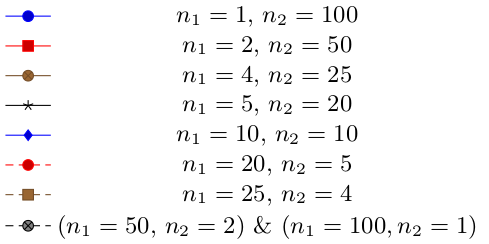
\includegraphics[scale=0.35]{Figs/Legend.png}
% \end{subfigure}
% \caption{Key Size ratio - Proposed Aggregate Scheme vs Hierarchical Scheme}
% \label{plot:keysize}
% \end{figure*}
% 
% Next, we compare specifically the key size required for the proposed extended scheme, for different values of $n_1$ and $n_2$ (again corresponding to $n=100$), with that required for a hierarchical encryption construction \cite{sandhu1988cryptographic}. Since our scheme uses a hierarchy depth of $2$, we use the same for the hierarchical construction as well, with $n_1$ nodes in level $0$, and $n_2$ level $1$ nodes in the subtree rooted at each level $0$ node. Figure \ref{plot:keysize} summarizes the findings. Evidently, lower the value of $n_1$, better the key aggregation, hence lower the ratio.
% 
% \subsection{Utilization Coefficient Comparison}
% \label{subsec:util}
% 
% Finally we compare the utilization-coefficient of the extended scheme for various values of $n_1$ and $n_2$ (corresponding to $n=100$) with increase in the number of registered key pairs $l$, where each key pair increases the number of classes by $n_2$. We leave out the configuration $n_1=n,n_2=1$ because that always leads to an utilization coefficient of $1$ but is impractical due to huge space requirements. Figure \ref{fig:util} demonstrates that that beyond a certain value of $l$, the combination $(1,n)$ proposed in \cite{chu2014key} has a lower utilization coefficient that all other combinations of $(n_1,n_2)$ for a given $n$. This emphasizes the advantage of making the choice of $(n_1,n_2)$ flexible.
% 
% \begin{figure*}[!t]
% \captionsetup{font=scriptsize}
% \centering
% \begin{subfigure}{0.5\textwidth}
% \captionsetup{font=scriptsize}
% \centering
% % \hspace{100.13cm}
% 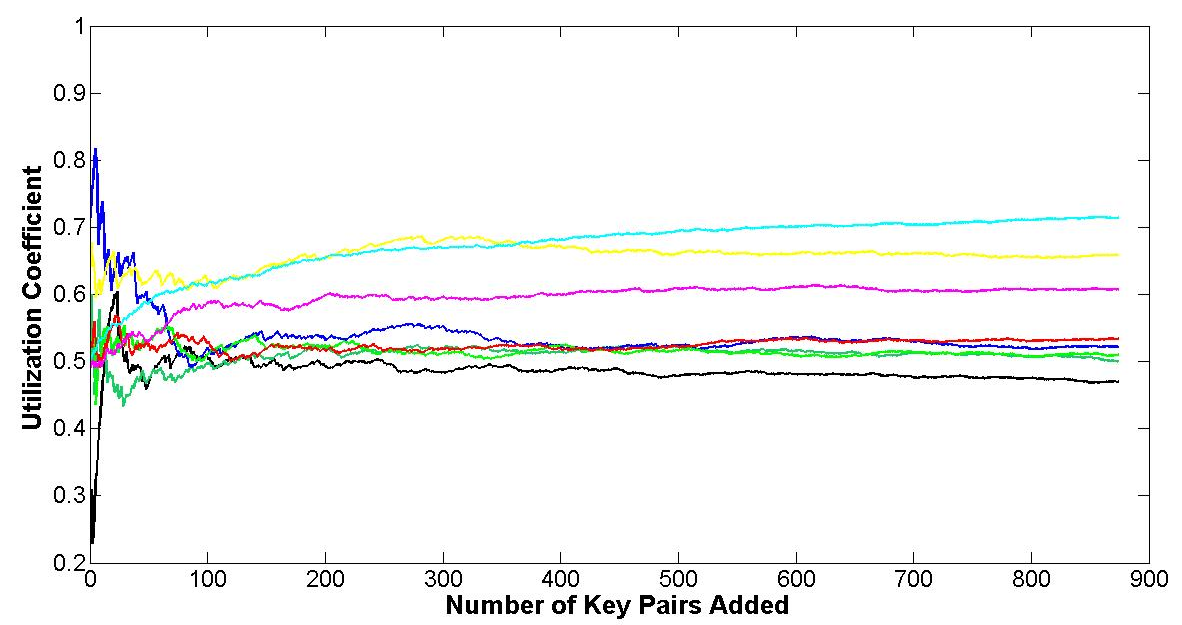
\includegraphics[scale=0.22]{Figs/UtilizationPlot.png}
% \end{subfigure}%
% \begin{subfigure}{0.5\textwidth}
% \captionsetup{font=scriptsize}
% \centering
% \hspace*{3.13 cm}
% 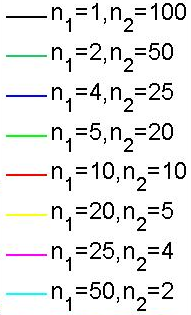
\includegraphics[scale=0.3]{Figs/Legend1.png}
% \end{subfigure}
% \caption{Utilization coefficient vs Newly Registered Keys}
% \label{fig:util}
% \end{figure*}
% 
